\section{SMEFT Parameterization}\label{sec:eft_parameterization}

\subsection{Overview and Assumptions}

The combination of input analyses is performed at the likelihood level~\cite{CMS-PAS-HIG-21-018}, and for the SMEFT interpretation, the probability distribution for the primary observables in each analysis, $p(\vec{x};\vec{\mu},\vec{\nu})$ (\cref{eq:statistical_model}), must be rewritten in terms of the SMEFT Wilson coefficients, $\vec{C}$.

Firstly, the probability distributions for the background processes are assumed to be independent of $\vec{C}$. This is a reasonable assumption since most background processes are constrained well by the data, e.g.\ in control regions. For the signal, every STXS bin (stage 0 or 1.2 depending on the analysis) is treated as a separate process, which for an analysis category, $c$, has an expected number of events given by:
\begin{equation}
  N_{pd}^c(\vec{C}) = \sigma^p(\vec{C}) \cdot \BR^d(\vec{C}) \cdot A_{pd}^c(\vec{C}) \cdot \mathcal{L}
  \label{eq:eft_expected_events}
\end{equation}
where $\sigma^p$ is the cross section for the STXS bin, $\BR^d$ is the branching fraction for the decay channel, $A_{pd}^c$ is the acceptance, and $\mathcal{L}$ is the integrated luminosity. Here, acceptance is taken to mean the fraction of events from a process that land in a particular analysis category.

In shape-based analyses, $p(\vec{x};\vec{\mu},\vec{\nu})$ also includes a description of the shape of the observable. In this interpretation, the shape is assumed to be independent of $\vec{C}$, and therefore, only the parameterization of $N_{pd}^c(\vec{C})$ is considered. This is a safe assumption for observables like the diphoton invariant mass whose shape is mainly driven by the experimental resolution of the CMS ECAL. For observables like a BDT output score, whose inputs could be e.g.\ the Higgs boson \pt, the assumption is less safe, but the assumption is kept since the SMEFT impact on the shape is still expected to be a second-order effect compared to the impact on the rate.

Furthermore, for all except the \Hfl and \Hlnulnu decay channels, the acceptance is also assumed to be independent of $\vec{C}$. The validity of this assumption and the special treatment applied to \Hfl and \Hlnulnu is discussed further in \cref{sec:acceptance_corrections}. For the rest of the channels, the SMEFT parameterization is reduced to determining $\sigma^p(\vec{C})$ and $\BR^d(\vec{C})$ for each STXS bin and decay channel respectively. 

Only single insertions of dimension-6 operators are considered, which leads to quadratic dependencies of $\sigma^p$ and $\Gamma^d$ on $\vec{C}$ (see \cref{sec:smeft_general_form}), where $\Gamma^d$ is the partial width for decay channel $i$, and the branching fractions are then expressed as $\Gamma^d(\vec{C}) / \Gamma^\PH(\vec{C})$ where $\Gamma^\PH$ is the total width of the Higgs boson. The total width parameterization is created by deriving the parameterization for all decay channels, including those not in \cref{tab:eft_input_channels}, and summing the widths: $\Gamma_H(\vec{C}) = \sum_d \Gamma^d(\vec{C})$. 

The SMEFT contributions to $\sigma^p$ and $\Gamma^d$ are assumed to factorize from NLO (and higher order) QCD and EW corrections so that one can write:
\begin{equation}
  \sigma^p(\vec{C}) = \sigma^p_{\text{SM}} \cdot \frac{\sigma^p_{\text{LO}}(\vec{C})}{\sigma^p_{\text{LO,SM}}}, \quad\quad \Gamma^d(\vec{C}) = \Gamma^d_{\text{SM}} \cdot \frac{\Gamma^d_{\text{LO}}(\vec{C})}{\Gamma^d_{\text{LO,SM}}}
  \label{eq:eft_nlo_lo_factorization}
\end{equation} 
where $\sigma^p_{\text{SM}}$ and $\Gamma^d_{\text{SM}}$ are the SM cross sections and decay widths calculated at the highest order available, $\sigma^p_{\text{LO,SM}}$ and $\Gamma^d_{\text{LO,SM}}$ are the same calculated at LO, and $\sigma^p_{\text{LO}}(\vec{C})$ and $\Gamma^d_{\text{LO}}(\vec{C})$ are the SMEFT equivalents, also calculated at LO. \Cref{eq:eft_nlo_lo_factorization} is usually written in terms of signal strengths, $\mu^p(\vec{C})$ and $\mu^d(\vec{C})$, which are defined as:
\begin{equation}
  \mu^p(\vec{C}) = \frac{\sigma^p_{\text{LO}}(\vec{C})}{\sigma^p_{\text{LO,SM}}}, \quad\quad \mu^d(\vec{C}) = \frac{\Gamma^d_{\text{LO}}(\vec{C})}{\Gamma^d_{\text{LO,SM}}}
\end{equation}
where the dependence of $\mu$ on $\vec{C}$ is given by:
\begin{equation}
  \mu^k(\vec{C}) = 1 + \sum_i A_i^k C_i + \sum_{ij} B_{ij}^k C_i C_j
  \label{eq:scaling_equation}
\end{equation}
where $i$ and $j$ run over the Wilson coefficients. Equations of the form given in \cref{eq:scaling_equation} are often called \textit{scaling equations}, and collectively, completely characterize the SMEFT parameterization. 

Finally, the parameterization is chosen to be derived in the Warsaw basis with the \topUtl flavour assumption and the \mWinput input parameter scheme (\cref{sec:EFT}), and only CP-even operators are considered because the STXS stage 1.2 bins are not sensitive to the differences between CP-even and CP-odd operators.

\subsection{General Methodology}\label{sec:eft_methodology_overview}
\begin{table}
  \caption[SMEFT Interpretation Methodology Overview]{Summary of techniques used to derive every scaling equation in the SMEFT interpretation. The \Hgg and \HZg equations are taken from analytical calculations described in Refs.~\cite{Dawson:2018liq,Dawson:2018pyl}. All other equations are derived via MC simulation, using either the \SMEFTsim or \SMEFTatNLO UFO models. The acceptance dependence on $\vec{C}$ is accounted for in the \Hfl and \Hlnulnu equations. The majority of the equations rely on event reweighting, with the exception of the inclusive (without acceptance corrections) \Hfl and \Hlnulnu equations that are used in the total width ($\PH\to\text{all}$) parameterization. Those equations are instead derived by generating dedicated samples at different values of $\vec{C}$.}
  \renewcommand{\arraystretch}{1.2}
  \begin{tabular}{@{}cccccc@{}}
  \toprule
  Method                               & Mode / Channel                           & UFO Model                     & Reweighting                    & Dedicated                      & \begin{tabular}[c]{@{}c@{}}Acceptance\\ corrections\end{tabular} \\ \midrule
  \multirow{2}{*}{MC}                  & \ggH                                     & \multirow{2}{*}{\SMEFTatNLO}  & \checkmark                     &                                &                                                                  \\
                                       & \ggZH                                    &                               & \checkmark                     &                                &                                                                  \\ \midrule
  \multirow{11}{*}{MC}                 & \qqH                                     & \multirow{11}{*}{\SMEFTsim}   & \checkmark                     &                                &                                                                  \\
                                       & \WH                                      &                               & \checkmark                     &                                &                                                                  \\
                                       & \ZH                                      &                               & \checkmark                     &                                &                                                                  \\
                                       & \bbH                                     &                               & \checkmark                     &                                &                                                                  \\
                                       & \ttH                                     &                               & \checkmark                     &                                &                                                                  \\
                                       & \tH                                      &                               & \checkmark                     &                                &                                                                  \\
                                       & \Hbb                                     &                               & \checkmark                     &                                &                                                                  \\
                                       & \Htautau                                 &                               & \checkmark                     &                                &                                                                  \\
                                       & \Hmumu                                   &                               & \checkmark                     &                                &                                                                  \\
                                       & \Hlnulnu                                 &                               & \checkmark                     &                                & \checkmark                                                                 \\
                                       & \Hfl                                     &                               & \checkmark                     &                                & \checkmark                                                       \\ \midrule
  \multirow{2}{*}{Analytical}          & \Hgg                                     & \multicolumn{4}{c}{\multirow{2}{*}{N/A}}                                                                                                                           \\
                                       & \HZg                                     & \multicolumn{4}{c}{}                                                                                                                                               \\ \midrule
                                       \begin{tabular}[c]{@{}c@{}}MC \&\\ analytical\end{tabular}            & $\PH \to \text{all}$ & \SMEFTsim                    & \checkmark  & \checkmark &                                                                  \\ \bottomrule
  \end{tabular}\label{tab:eft_derivation_summary}
\end{table}

The scaling equations are derived with a mixture of techniques, summarized in \cref{tab:eft_derivation_summary}, which depend on the production mode and decay channel. The scaling equations are determined entirely via MC simulation, with the exception of the \Hgg and \HZg partial widths. These equations are instead taken from analytical calculations provided in Refs.~\cite{Dawson:2018liq} and~\cite{Dawson:2018pyl} respectively, where a conversion is applied to the \topUtl basis. These processes are the exceptions because they both contain an electroweak loop in their LO Feynman diagrams and this type of diagram cannot be computed in the SMEFT with currently-available MC tools.

To derive a scaling equation using MC simulation, the corresponding cross section or partial width is calculated at LO using different values of the Wilson coefficients, and the $A$ and $B$ terms are inferred. For $N$ Wilson coefficients, the cross section or partial width must be calculated at $2N + (N-1)/2$ points in the Wilson coefficient space to determine all terms. 

A cross section/partial width is calculated by first generating events for the corresponding process using \MADGRAPH v2.6.7~\cite{MadGraph,MadGraphMLM} where the SM is assumed. For a partial width, the sum of weights from these events corresponds to $\Gamma^d(\vec{C}=0)$. If a cross section is being calculated, the events are interfaced with \PYTHIA 8.306~\cite{Sjostrand:2014zea} with the CP5 tune~\cite{CMS:2015wcf,CMS:2019csb} for parton showering and fragmentation before being categorized into the STXS bins by a \rivet~\cite{Bierlich:2019rhm} routine. Then, the sum of event weights in an STXS bin corresponds to the value of $\sigma^p(\vec{C}=0)$.

Two UFO (Universal FeynRules Output)~\cite{Degrande:2011ua} models are used to implement the SMEFT contributions in the \MADGRAPH simulations. The \SMEFTatNLO~\cite{Degrande:2020evl} model is capable of calculating SMEFT contributions at NLO in QCD and is used for the loop-induced \ggH and \ggZH processes. Alternatively, \ggH could be simulated using LO UFO models like \SMEFTsim, but this relies on an EFT (not SMEFT) approximation of the process which breaks down for $\ptH > m_\Pqt$~\cite{Brivio:2020onw}, and neglects SMEFT contributions that enter via the top-quark loop (see left of \cref{fig:ggH_feynman}). In all cases apart from \ggH and \ggZH, the \SMEFTsim model is used, and is preferred over \SMEFTatNLO in these cases because it also includes propagator corrections (see \cref{sec:h4l_eft_theory}).

Using these UFO models, the partial widths and cross sections for different values of $\vec{C}$ are mainly determined by reweighting the events~\cite{Mattelaer:2016gcx} and then summing the new weights as before. This is a fair method when only minor changes to the phase space are expected due to the SMEFT contributions, where here, phase space means the components of all outgoing particle four-momenta. If a SMEFT contribution leads to an area of phase space being far more likely than in the SM, then a large SMEFT contribution will be described by a small number of events, leading to a large statistical uncertainty. This ultimately translates into an uncertainty in the $A$ and $B$ terms.

In the final result extraction, the uncertainties on the $A$ and $B$ terms are neglected so it is important that they remain small. However, there are cases, like that described in \cref{sec:h4l_eft_theory} for \Hfl, where high uncertainties are expected, and are indeed found. For example, in an equation derived using $10^5$ reweighted events for the $\PH \to 4e$ partial width, the $A$ term for the $Q_{HW}$ operator had an uncertainty of 740\%. This cannot be neglected and generating enough events to reduce this uncertainty to a reasonable level would be too computationally expensive.

A similar level of uncertainty was found in the other $\PH \to 4f$ channels: \Hlnulnu, $\PH \to llqq$, $\PH \to \nu\nu qq$, $\PH \to qqqq$, specifically for the $Q_{HW}$, $Q_{HB}$ and $Q_{HWB}$ operators. Therefore, in these channels, the terms involving these operators are not determined by reweighting. Instead, the relevant partial widths are calculated by re-generating events (dedicated events) at the appropriate Wilson coefficient values. This leads to $<10\%$ uncertainty in all the corresponding terms. 

In \cref{tab:eft_derivation_summary}, one might have noticed that the \Hfl is not indicated to use dedicated generation, which seems contradictory to the discussion above. This is because two scaling equations are derived for \Hfl, one which corresponds to the inclusive partial width and one that corresponds to a fiducial partial width. The former is used in a calculation of the total width, and does require dedicated generation, hence why the total width is indicated to use dedicated generation in \cref{tab:eft_derivation_summary}. The latter is used to parameterize $N_{pd}^c$ for the \Hfl channel, and does not require dedicated generation for reasons related to acceptance corrections which are discussed in \cref{sec:acceptance_corrections}. For the same reasons, \Hlnulnu is also not indicated to use dedicated generation in \cref{tab:eft_derivation_summary}.

\subsection{Acceptance Corrections}\label{sec:acceptance_corrections}

In the \Hfl analysis~\cite{CMS:2021ugl}, opposite-charge, same-flavour lepton pairs are formed and a selection of $12 < \mll < 120$\GeV is placed. For \Hfl events, one pair of leptons typically comes from an on-shell \PZ boson ($\mZ \sim 91\GeV$) and is therefore likely to pass this selection. The invariant mass of the pair of leptons whose mass is the furthest away from \mZ is denoted \mthreefour, and the distribution of this variable in simulated \Hfl events is shown in \cref{fig:h4l_m34}. The distribution is shown for the SM and also for $C_{HB}=0.5$. A significant enhancement is seen at low values of \mthreefour, which is explained by the SMEFT Feynman diagrams shown in \cref{fig:H4l_feynman_za}, that introduce a term like $1/\mthreefour^2$ to the matrix element. Given that the shape of the \mthreefour distribution depends on the SMEFT, and that the analysis criteria places a cut on this variable, the acceptance, $A$, is dependent on $\vec{C}$.

\begin{figure}
  \centering
  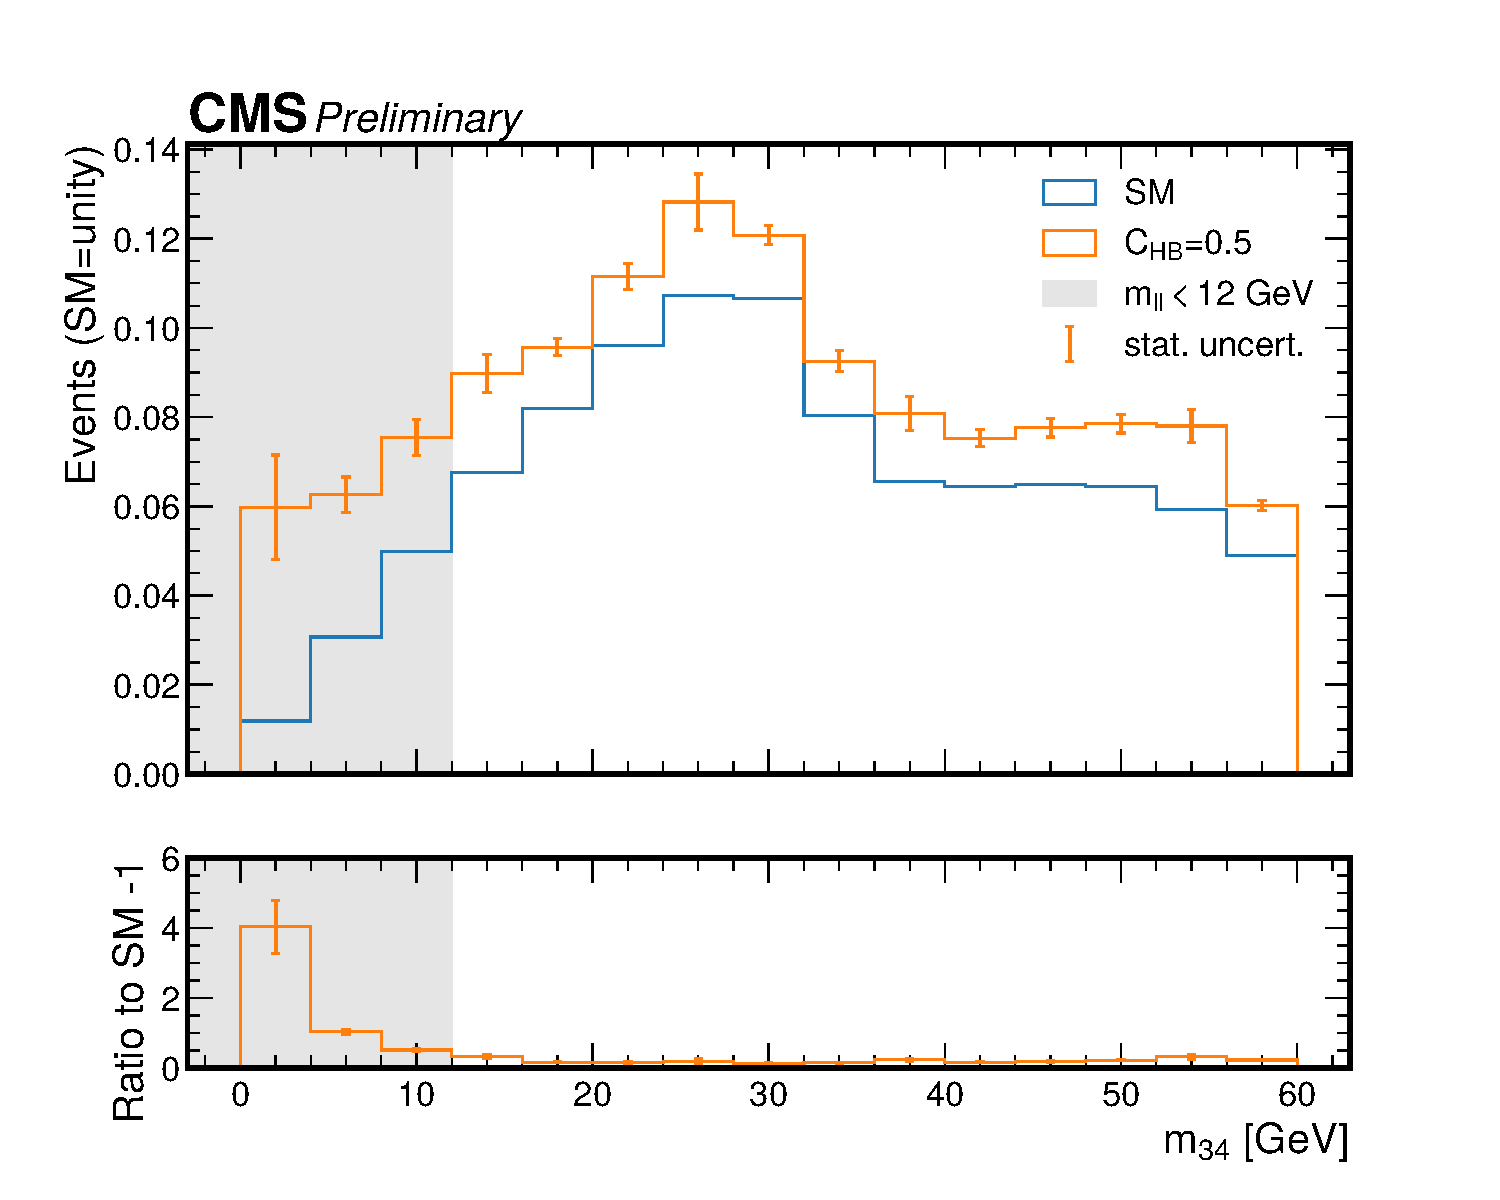
\includegraphics[width=0.9\textwidth]{Figures/EFT/H4l_m34_CMS.pdf}
  \caption[Distribution of \mthreefour in the SM and in the SMEFT with $C_{HB}=0.5$]{Distribution of \mthreefour in the SM (blue) and in the SMEFT with $C_{HB}=0.5$ (orange). The additional contribution from the SMEFT relative to the SM is shown in the bottom plot where the largest contribution is seen at the smallest values of \mthreefour.}\label{fig:h4l_m34}
\end{figure}

So far, the \Hfl scaling equation has been derived by considering the SMEFT contribution to all \Hfl events (inclusively). To account for the acceptance dependence, the scaling equation for \Hfl is derived using only the events that pass the analysis selection. In this way, the scaling equation for the \Hfl branching fraction accounts for the acceptance dependence and a separate equation for the acceptance is not needed. 

Practically, this is achieved by reusing the simulated datasets originally used by the analysis, applying the selection criteria, and then reweighting the remaining events using a standalone reweighting tool~\cite{nanoAODtools,Mattelaer:2016gcx}. Reweighting is a valid approach here because the previously problematic region of phase space ($1/\mll^2 \sim 0$) is removed by the selection criteria. 

These datasets were generated with the full CMS simulation chain, including the detector response modelled with the \GEANTfour package~\cite{Agostinelli:2002hh}, and the object reconstruction. This is important because repeating a similar derivation by applying the selection criteria to generator-level quantities could lead to different (less valid) results if, for example, the experimental resolution on \mthreefour was particularly poor. 

The inclusive and acceptance-corrected \Hfl partial width scaling is shown in \cref{fig:h4l_acceptance_corrected} as functions of the Wilson coefficients whose $A$ and $B$ terms change the most after considering acceptance corrections. These coefficients are $C_{HB}$, $C_{HW}$ and $C_{HWB}$, which is expected since they all give rise to Feynman diagrams shown in \cref{fig:H4l_feynman_za}. At values of $C = 1$, the scaling of the partial width is different up to a factor of 5, illustrating the need for acceptance corrections for the \Hfl decay. Similarly, selection criteria placed in the \Hlnulnu analysis~\cite{CMS:2022uhn} can also lead to acceptance dependence and the scaling equation for the \Hlnulnu partial width is derived using the same methods.

\begin{figure}
  \centering
  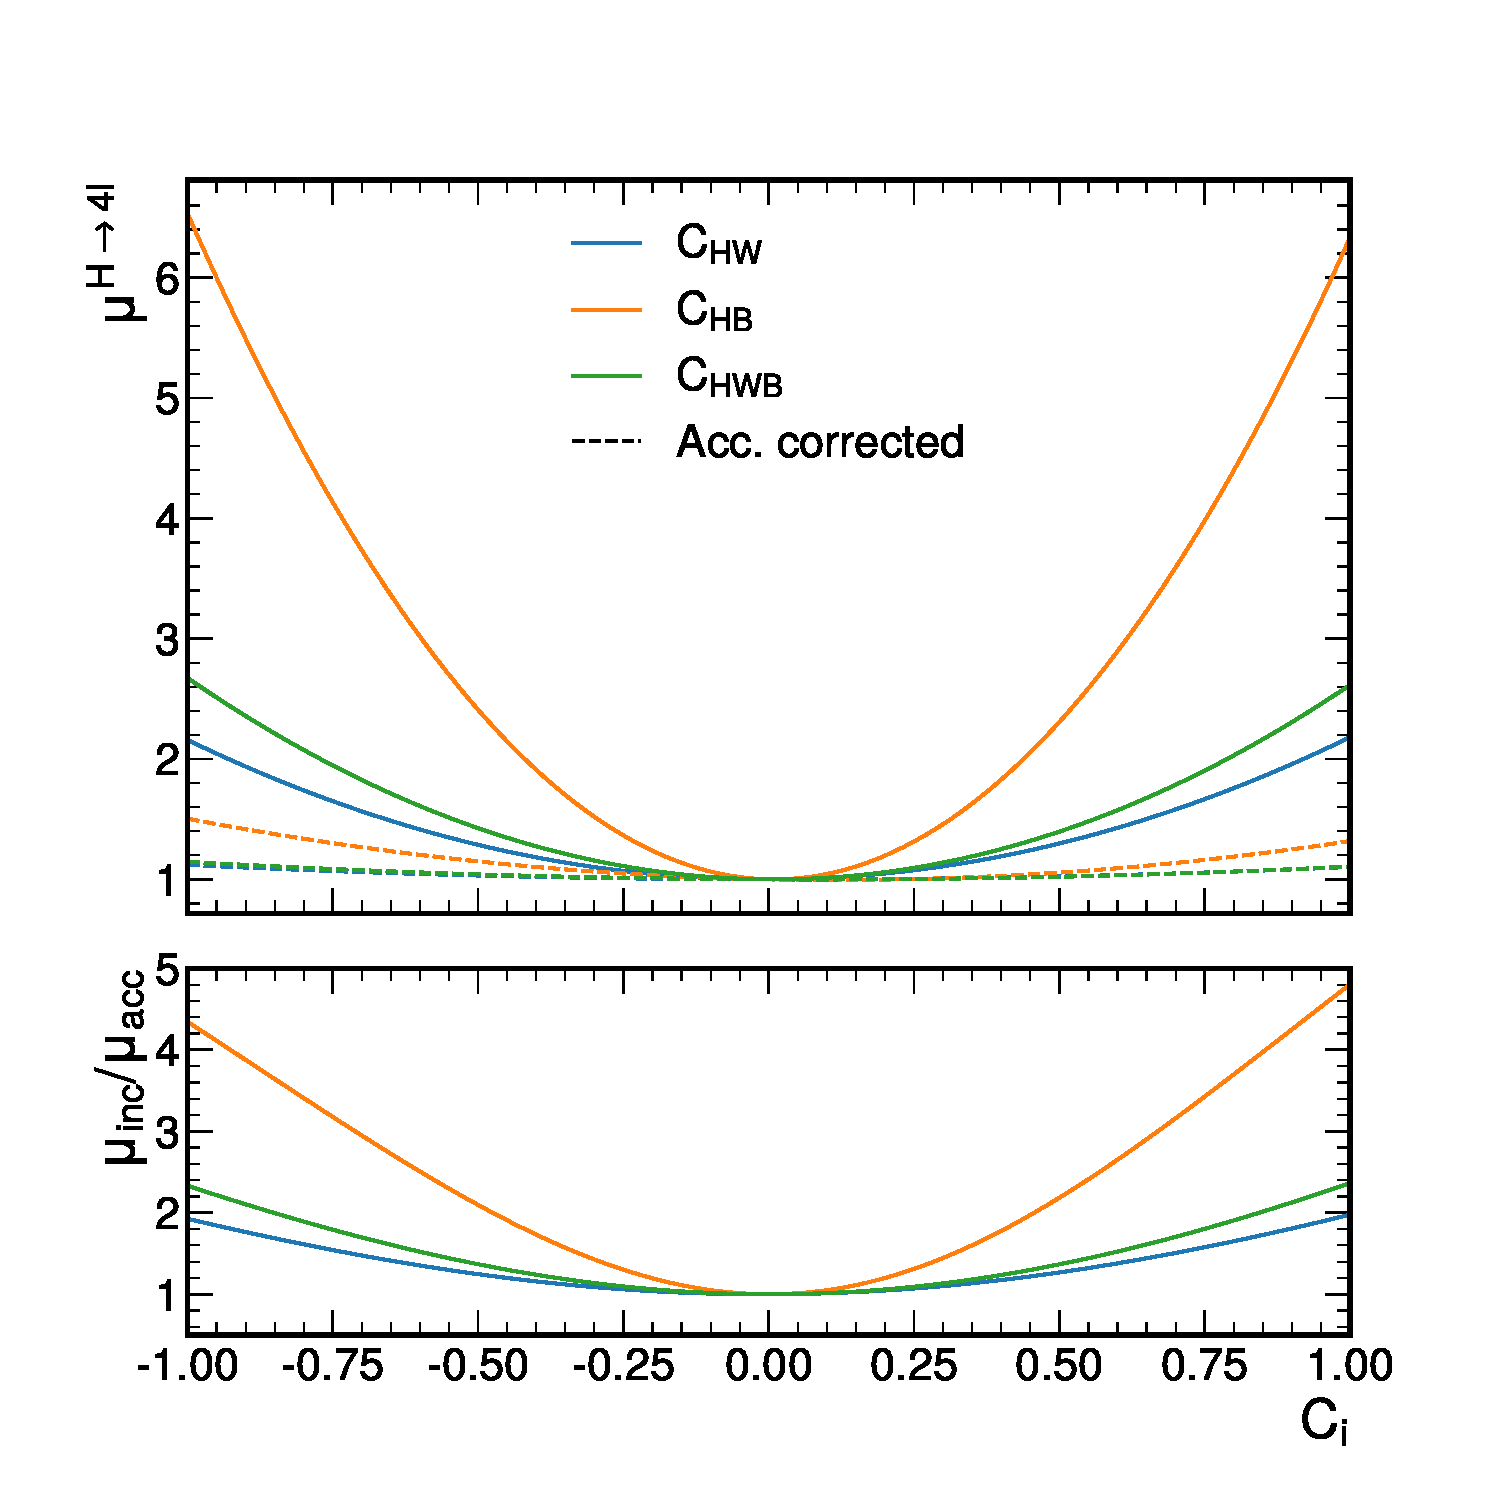
\includegraphics[width=0.7\textwidth]{Figures/EFT/h4l_acc_corr.pdf}
  \caption[Impact of Acceptance Corrections on the \Hfl Partial Width]{Scaling of the \Hfl partial width as functions of $C_{HW}$, $C_{HB}$, and $C_{HWB}$. The solid and dashed lines show the scaling equation when not considering acceptance corrections (an inclusive calculation), and when acceptance corrections are applied, respectively. The ratio of these two equations is shown in the bottom plot.}\label{fig:h4l_acceptance_corrected}
\end{figure}

In the two-body decays, the decay products must always decay back-to-back and with energy $\mH / 2$ in the Higgs boson rest frame. Therefore, SMEFT contributions cannot change the distribution of any kinematic variable related to the decay and there cannot be acceptance corrections. Hence, deriving the scaling equations with the approaches described in this subsection is unnecessary for the two-body decays.

Considering now the different production modes and their cross sections, there is the possibility that acceptance corrections are required. Selected criteria are often placed, for example, on \ptH, and this is a variable whose distribution can be changed in the SMEFT. However, the STXS is binned in the variables whose distributions are expected to change the most from new physics contributions, like \ptH. Therefore, for the scaling equation for a particular STXS bin, the analysis criteria are already well aligned with the events being used to derive the equation, at least in the variables that would lead to acceptance dependence. So, any acceptance dependence related to production is expected to be small and is neglected.

\subsection{Summary}
The parameterization of the Higgs boson cross sections and the decay widths are derived up to quadratic order in the Wilson coefficients. The rate of a process, which is a product of the cross sections and branching fractions, is then Taylor expanded up to quadratic order in the Wilson coefficients to isolate the contributions which are suppressed by $1/\Lambda^2$ (linear terms) and $1/\Lambda^4$ (quadratic terms), and to exclude terms suppressed by higher orders which are expected to be small. Furthermore, only the significant terms from the expansion are kept by removing terms where $\abs{A}$ or $\abs{B}$ is less than 0.01. This is reasonable because none of the measurements are made to greater than a few percent precision, so they cannot be sensitive to these Wilson coefficients unless $C \gg \mathcal{O}(1)$, in which case the EFT expansion is no longer valid anyway. The resulting parameterization has 43 different Wilson coefficients which are listed in \cref{tab:wilson_coeffs_43}.

The impacts of the Wilson coefficients on the STXS and Higgs boson branching fractions are shown in \cref{fig:smeft_parametrisation_part1,fig:smeft_parametrisation_part2,fig:smeft_parametrisation_part3}. As discussed in \cref{sec:EFT}, there are different classes of contributions. The $C_{H \square}$ coefficient enters every process and scales them by an equal amount (purple in top quarter of \cref{fig:smeft_parametrisation_part1}). Then, there are contributions that primarily affect a single process, such as $C_{HG}$ for \ggH (blue in top-middle quarter of \cref{fig:smeft_parametrisation_part1}), or the four-fermion Wilson coefficients for the \ttH process (\cref{fig:smeft_parametrisation_part3}). These sorts of contributions highlight the importance of combining as many different processes as possible. Finally, there are contributions than benefit from the STXS binning, such as $C_{Hq}^{(3)}$ for the $\VH$ processes (\cref{fig:smeft_parametrisation_part2}) where the high $\pt^\PV$ bins are more sensitive to this coefficient.

\begin{table}
    \centering
    \caption[Contributing Wilson Coefficients to SMEFT Interpretation]{A list of the 43 Wilson coefficients and their associated operators that the SMEFT interpretation is sensitive to. 
             This table is a subset of \cref{tab:Warsaw_basis,tab:topU3l_basis} that provide the full set of operators in the Warsaw basis under the \topUtl flavour assumption.
             Table taken from Ref.~\cite{CMS-PAS-HIG-21-018}.}\label{tab:wilson_coeffs_43}
    \centering
    \footnotesize
    \renewcommand{\arraystretch}{1.5}

    \begin{minipage}[t]{0.49\textwidth}
        \vspace{0pt}
        \resizebox{0.95\linewidth}{!}{
            \centering
            \begin{tabular}{l|c|c}
                \toprule
                Group $\qquad$                    & WC                    & Operator                                                                          \\
                \midrule
                \multirow{2}{*}{$X^3$}            & $c_W$                 & $\epsilon^{ijk}W^{i\nu}_{\mu}W^{j\rho}_{\nu}W^{k\mu}_{\rho}$                      \\
                                                  & $c_G$                 & $f^{abc}G^{a\nu}_{\mu}G^{b\rho}_{\nu}G^{c\mu}_{\rho}$                             \\
                \midrule
                \multirow{2}{*}{$H^4D^2$}         & $c_{H\Box}$           & $(H^{\dagger}H)\Box(H^{\dagger}H)$                                                \\
                                                  & $c_{HD}$              & $(D^{\mu}H^{\dagger}H)(H^{\dagger}D^{\mu}H)$                                      \\
                \midrule
                \multirow{2}{*}{$X^2H^2$}         & $c_{HG}$              & $H^{\dagger}HG^{a}_{\mu\nu}G^{a,\mu\nu}$                                          \\
                                                  & $c_{HW}$              & $H^{\dagger}HW^{i}_{\mu\nu}W^{i,\mu\nu}$                                          \\
                                                  & $c_{HB}$              & $H^{\dagger}HB_{\mu\nu}B^{\mu\nu}$                                                \\
                                                  & $c_{HWB}$             & $H^{\dagger}HW^{i}_{\mu\nu}B^{\mu\nu}$                                            \\
                \midrule
                \multirow{3}{*}{$\psi^2H^3$}      & $\mathrm{Re}(c_{eH})$ & $(H^{\dagger}H)(\bar{l}_p e_r H)$                                                 \\
                                                  & $\mathrm{Re}(c_{bH})$ & $(H^{\dagger}H)(\bar{Q} \tilde{H} t)$                                             \\
                                                  & $\mathrm{Re}(c_{tH})$ & $(H^{\dagger}H)(\bar{Q}Hb)$                                                       \\
                \midrule
                \multirow{5}{*}{$\psi^2{X}H$}     & $\mathrm{Re}(c_{tG})$ & $(\bar{Q}\sigma^{\mu\nu}{T^a}t)\tilde{H}G^a_{\mu\nu}$                             \\
                                                  & $\mathrm{Re}(c_{tW})$ & $(\bar{Q}\sigma^{\mu\nu}t)\sigma^i\tilde{H}W^i_{\mu\nu}$                          \\
                                                  & $\mathrm{Re}(c_{tb})$ & $(\bar{Q}\sigma^{\mu\nu}t)\tilde{H}B_{\mu\nu}$                                    \\
                                                  & $\mathrm{Re}(c_{bG})$ & $(\bar{Q}\sigma^{\mu\nu}{T^a}b)HG^a_{\mu\nu}$                                     \\
                                                  & $\mathrm{Re}(c_{bW})$ & $(\bar{Q}\sigma^{\mu\nu}b)\sigma^i{H}W^i_{\mu\nu}$                                \\
                \midrule
                \multirow{6}{*}{$\psi^2{H}^2{D}$} & $c^{(1)}_{Hl}$        & $(H^{\dagger}i\overleftrightarrow{D}_{\mu}H)(\bar{l}_p \gamma^\mu l_r)$           \\
                                                  & $c^{(3)}_{Hl}$        & $(H^{\dagger}i\overleftrightarrow{D}^i_{\mu}H)(\bar{l}_p \sigma^i\gamma^\mu l_r)$ \\
                                                  & $c^{(1)}_{Hq}$        & $(H^{\dagger}i\overleftrightarrow{D}_{\mu}H)(\bar{q} \gamma^\mu q)$               \\
                                                  & $c^{(3)}_{Hq}$        & $(H^{\dagger}i\overleftrightarrow{D}^i_{\mu}H)(\bar{q} \sigma^i\gamma^\mu q)$     \\
                                                  & $c^{(1)}_{HQ}$        & $(H^{\dagger}i\overleftrightarrow{D}_{\mu}H)(\bar{Q} \gamma^\mu Q)$               \\
                                                  & $c^{(3)}_{HQ}$        & $(H^{\dagger}i\overleftrightarrow{D}^i_{\mu}H)(\bar{Q} \sigma^i\gamma^\mu Q)$     \\
                \bottomrule
            \end{tabular}
        }
    \end{minipage}
    \hfill
    \begin{minipage}[t]{0.49\textwidth}
        \vspace{0pt}
        \resizebox{0.95\linewidth}{!}{
            \centering
            \begin{tabular}{l|c|c}
                \toprule
                Group $\qquad$                          & WC                     & Operator                                                                \\
                \midrule
                \multirow{6}{*}{$\psi^2{H}^2{D}$}       & $c_{He}$               & $(H^{\dagger}i\overleftrightarrow{D}_{\mu}H)(\bar{e}_p \gamma^\mu e_r)$ \\
                                                        & $c_{Hu}$               & $(H^{\dagger}i\overleftrightarrow{D}_{\mu}H)(\bar{u} \gamma^\mu u)$     \\
                                                        & $c_{Hd}$               & $(H^{\dagger}i\overleftrightarrow{D}_{\mu}H)(\bar{d} \gamma^\mu d)$     \\
                                                        & $\mathrm{Re}(c_{Htb})$ & $i(H^{\dagger}{D}_{\mu}H)(\bar{t} \gamma^\mu b)$                        \\
                                                        & $c_{Ht}$               & $(H^{\dagger}i\overleftrightarrow{D}_{\mu}H)(\bar{t} \gamma^\mu t)$     \\
                                                        & $c_{Hb}$               & $(H^{\dagger}i\overleftrightarrow{D}_{\mu}H)(\bar{b} \gamma^\mu b)$     \\
                \midrule
                \multirow{5}{*}{$(\bar{L}L)(\bar{L}L)$} & $c^{(1)}_{ll}$         & $(\bar{l}_p \gamma_\mu l_r)(\bar{l}_s \gamma^\mu l_t)$                  \\
                                                        & $c^{(11)}_{Qq}$        & $(\bar{Q} \gamma_\mu Q)(\bar{q} \gamma^\mu q)$                          \\
                                                        & $c^{(18)}_{Qq}$        & $(\bar{Q} T^a\gamma_\mu Q)(\bar{q} T^a\gamma^\mu q)$                    \\
                                                        & $c^{(31)}_{Qq}$        & $(\bar{Q} \sigma^i\gamma_\mu Q)(\bar{q} \sigma^i\gamma^\mu q)$          \\
                                                        & $c^{(38)}_{Qq}$        & $(\bar{Q} \sigma^iT^a\gamma_\mu Q)(\bar{q} \sigma^iT^a\gamma^\mu q)$    \\
                \midrule
                \multirow{4}{*}{$(\bar{R}R)(\bar{R}R)$} & $c^{(1)}_{tu}$         & $(\bar{t} \gamma_\mu t)(\bar{u} \gamma^\mu u)$                          \\
                                                        & $c^{(8)}_{tu}$         & $(\bar{t} T^a\gamma_\mu t)(\bar{u} T^a\gamma^\mu u)$                    \\
                                                        & $c^{(1)}_{td}$         & $(\bar{t} \gamma_\mu t)(\bar{d} \gamma^\mu d)$                          \\
                                                        & $c^{(8)}_{td}$         & $(\bar{t} T^a\gamma_\mu t)(\bar{d} T^a\gamma^\mu d)$                    \\
                \midrule
                \multirow{6}{*}{$(\bar{L}L)(\bar{R}R)$} & $c^{(1)}_{qt}$         & $(\bar{q} \gamma_\mu q)(\bar{t} \gamma^\mu t)$                          \\
                                                        & $c^{(8)}_{qt}$         & $(\bar{q} T^a\gamma_\mu q)(\bar{t} T^a\gamma^\mu t)$                    \\
                                                        & $c^{(1)}_{Qu}$         & $(\bar{Q} \gamma_\mu Q)(\bar{u} \gamma^\mu u)$                          \\
                                                        & $c^{(8)}_{Qu}$         & $(\bar{Q} T^a\gamma_\mu Q)(\bar{u} T^a\gamma^\mu u)$                    \\
                                                        & $c^{(1)}_{Qd}$         & $(\bar{Q} \gamma_\mu Q)(\bar{d} \gamma^\mu d)$                          \\
                                                        & $c^{(8)}_{Qd}$         & $(\bar{Q} T^a\gamma_\mu Q)(\bar{d} T^a\gamma^\mu d)$                    \\
                \bottomrule
            \end{tabular}
        }
    \end{minipage}



    
\end{table}


\begin{landscape}
  \begin{figure}
    \centering
    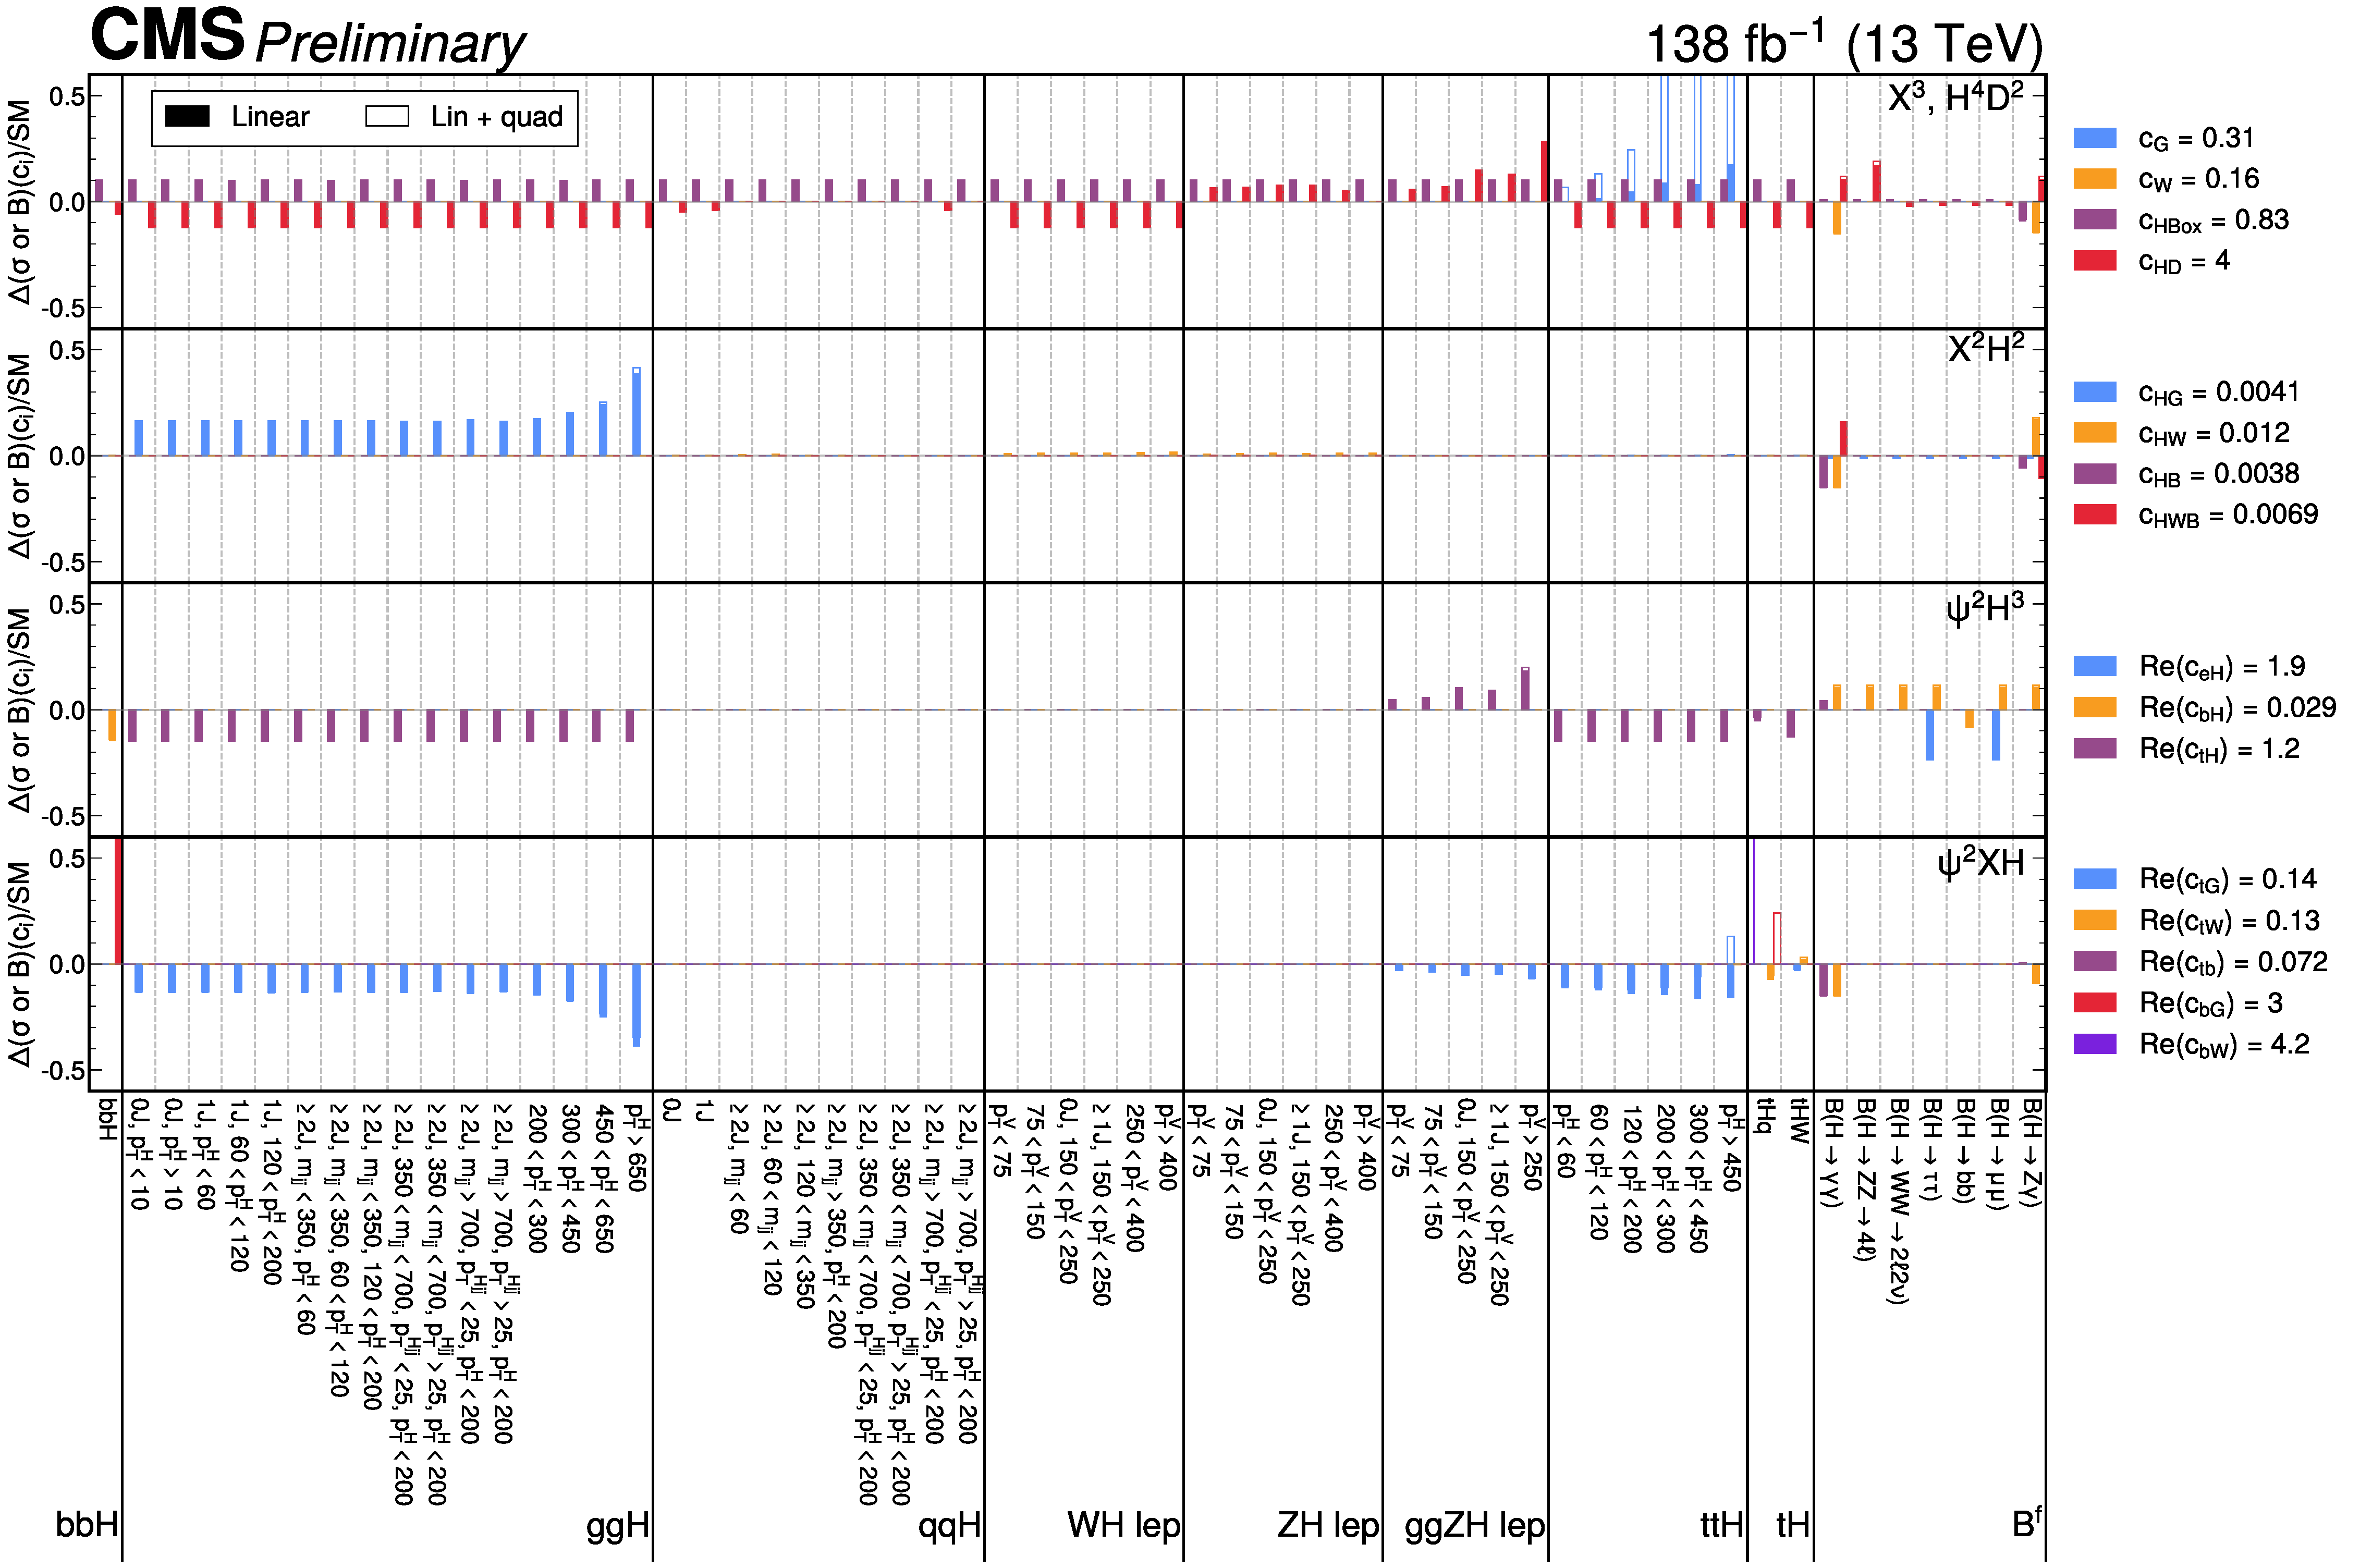
\includegraphics[width=\pagewidth]{Figures/EFT/HIG-21-018-Figure_014.pdf}
      \caption[Impact of SMEFT Operators in the SMEFT Basis (1)]{Impact of the SMEFT operators on the STXS and Higgs boson branching fractions. The impacts are shown for operators from the following groups: $X^3$, $H^4D^2$, $X^2H^2$, $\psi^2H^3$ and $\psi^2XH$ (see \cref{tab:Warsaw_basis,tab:topU3l_basis}). The Wilson coefficients are set to the expected symmetrized 95\% CL interval value, assuming all other Wilson coefficients are set to zero (SM). The impacts are presented relative to the SM prediction and are shown by the unfilled bars, and by the filled bars when considering only the linear ($A$) terms.}\label{fig:smeft_parametrisation_part1}
  \end{figure}
\end{landscape}

\begin{landscape}
  \begin{figure}
    \centering
    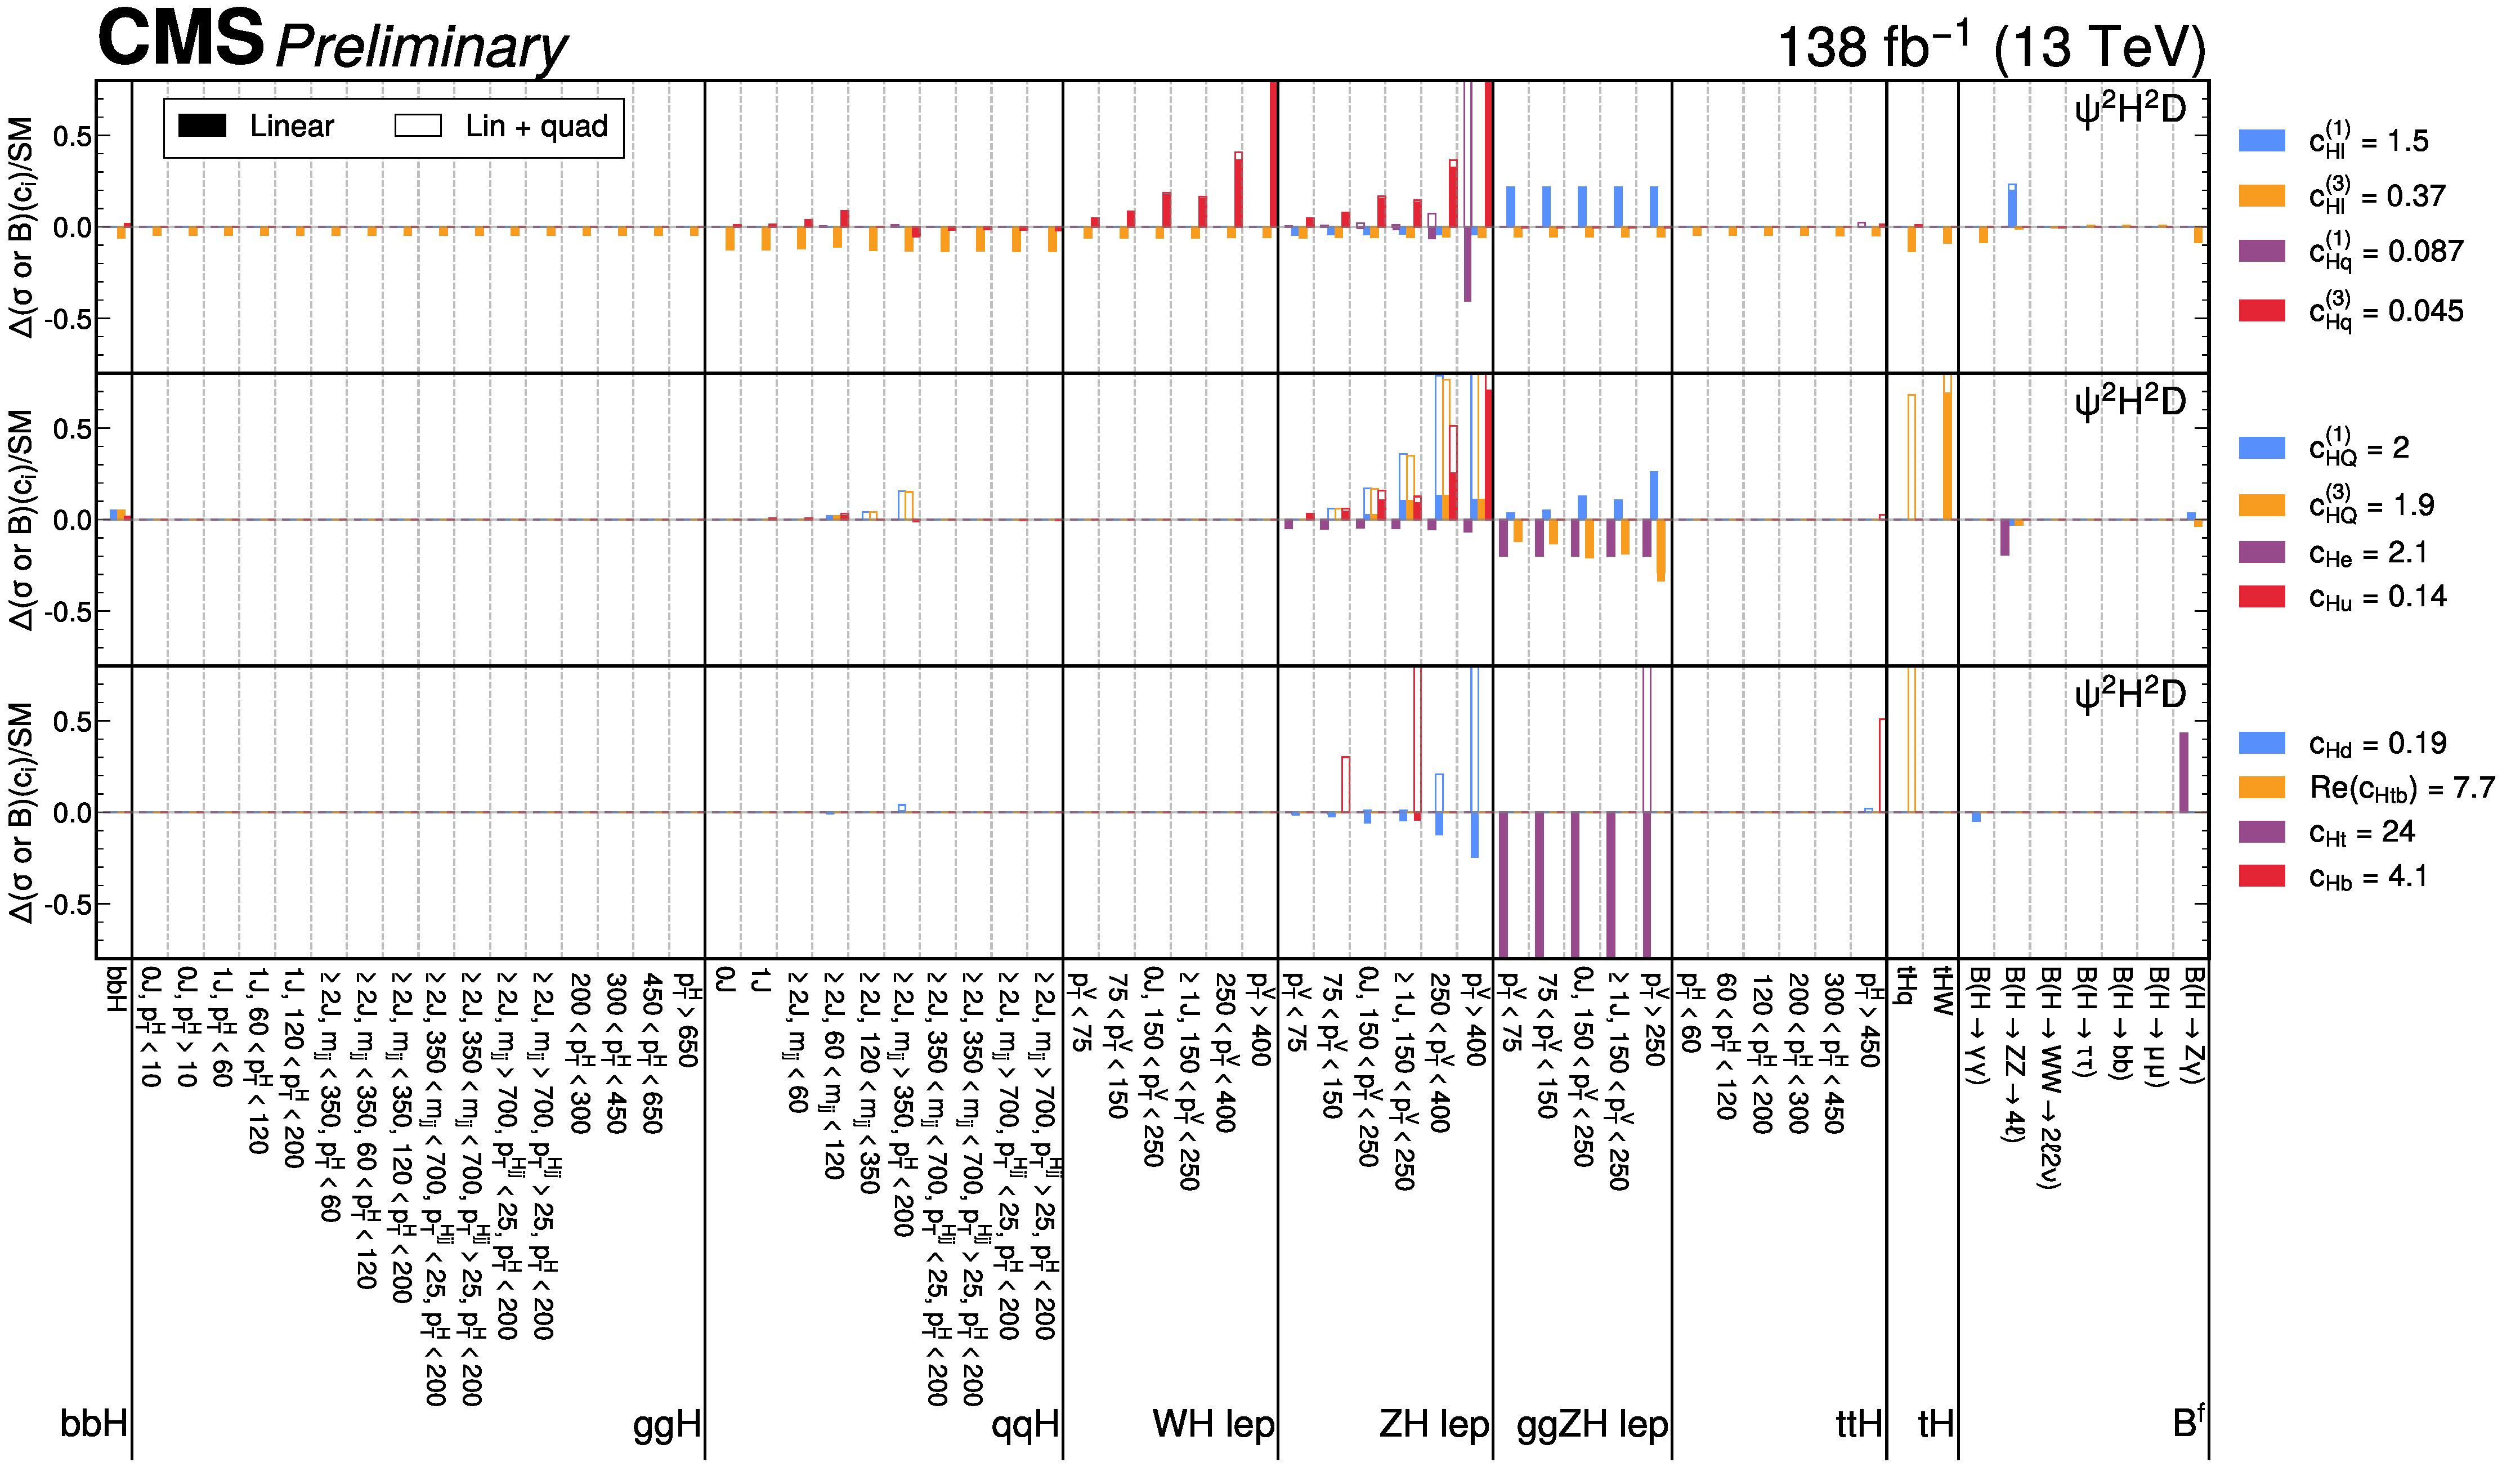
\includegraphics[width=\pagewidth]{Figures/EFT/HIG-21-018-Figure_015.pdf}
    \caption[Impact of SMEFT Operators in the SMEFT Basis (2)]{Impact of the SMEFT operators on the STXS and Higgs boson branching fractions. The impacts are shown for operators from the $\psi^2H^2D$ group (see \cref{tab:Warsaw_basis,tab:topU3l_basis}). The Wilson coefficients are set to the expected symmetrized 95\% CL interval value, assuming all other Wilson coefficients are set to zero (SM). The impacts are presented relative to the SM prediction and are shown by the unfilled bars, and by the filled bars when considering only the linear ($A$) terms.}\label{fig:smeft_parametrisation_part2}
  \end{figure}
\end{landscape}

\begin{landscape}
  \begin{figure}
    \centering
    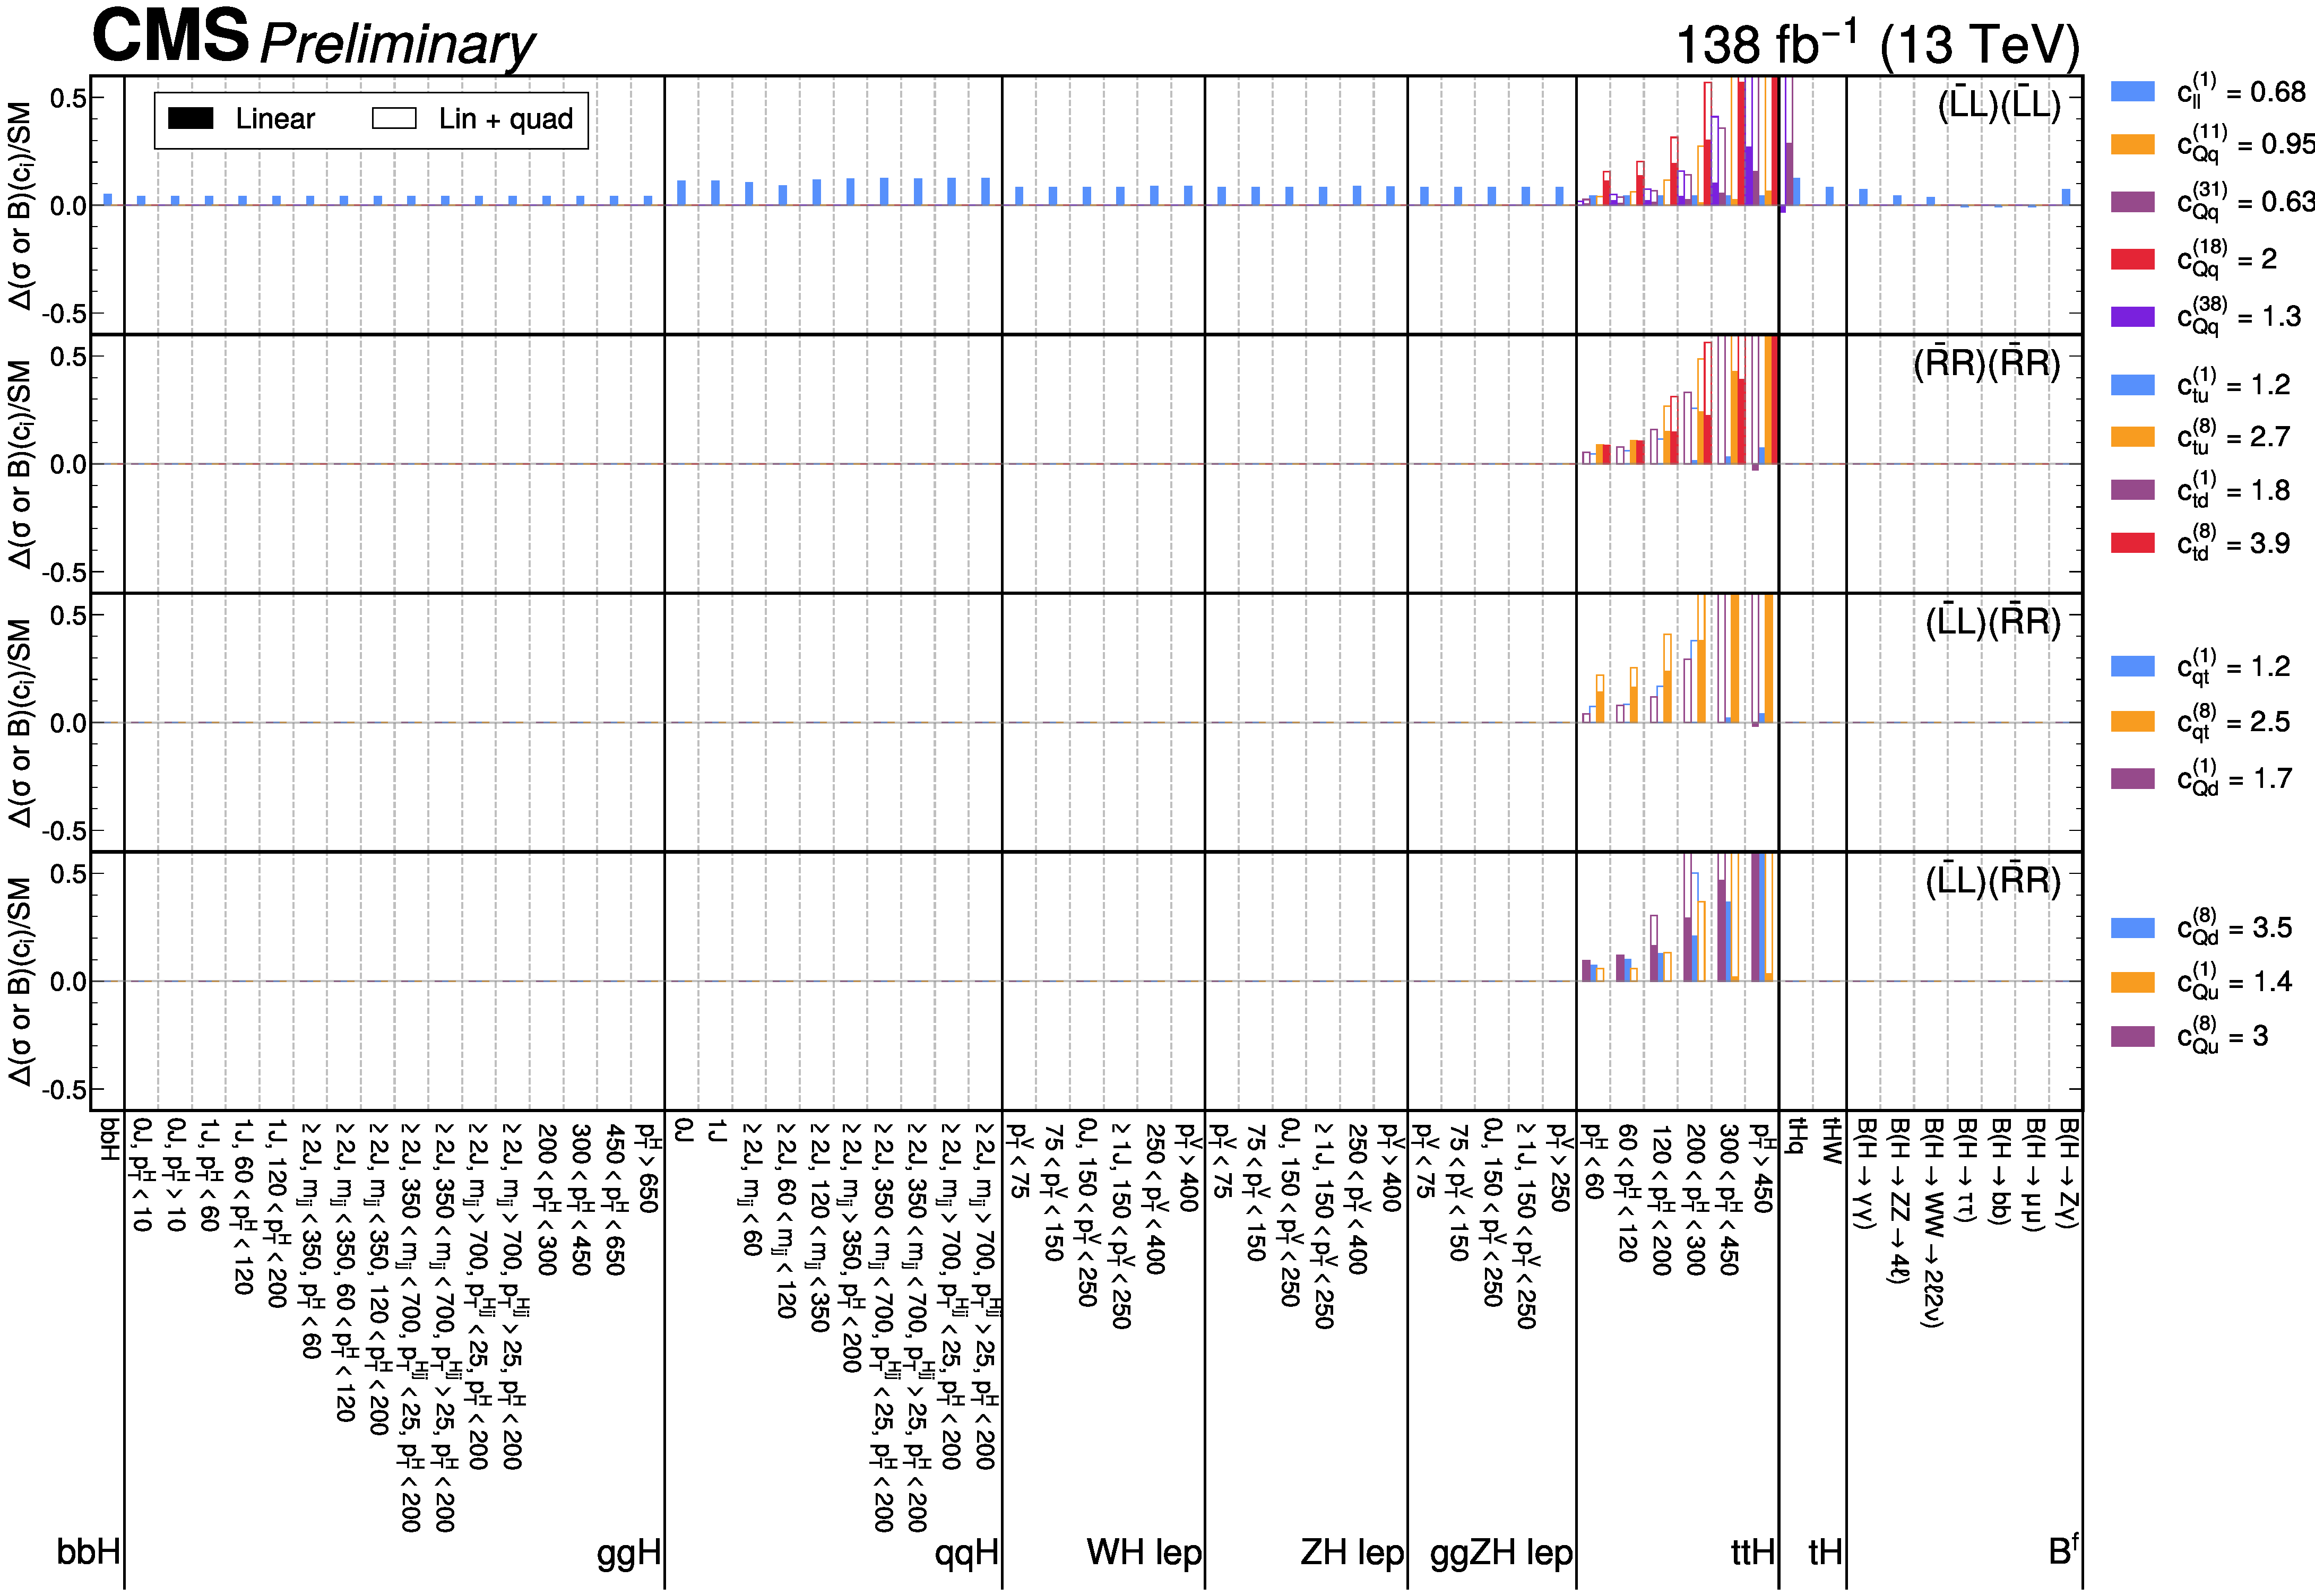
\includegraphics[width=\pagewidth]{Figures/EFT/HIG-21-018-Figure_016.pdf}
    \caption[Impact of SMEFT Operators in the SMEFT Basis (3)]{Impact of the SMEFT operators on the STXS and Higgs boson branching fractions. The impacts are shown for operators from the four-fermion groups (see \cref{tab:Warsaw_basis,tab:topU3l_basis}). The Wilson coefficients are set to the expected symmetrized 95\% CL interval value, assuming all other Wilson coefficients are set to zero (SM). The impacts are presented relative to the SM prediction and are shown by the unfilled bars, and by the filled bars when considering only the linear ($A$) terms.}\label{fig:smeft_parametrisation_part3}
  \end{figure}
\end{landscape}